\documentclass[sigconf,anonymous]{acmart}
\settopmatter{printacmref=false, printccs=true, printfolios=true}

% = = = ACM Metadata
%\setcopyright{acmcopyright}
%\copyrightyear{2018}
%\acmYear{2018}
%\acmDOI{10.1145/1122445.1122456}
\acmConference[SigITE '21]{SIGITE 2021 – 22nd Annual Conference on IT Education}{October 06--09, 2021}{Snowbird, UT}
\acmBooktitle{SIGITE 2021 – 22nd Annual Conference on IT Education, October 06--09, 2021, Snowbird, UT}
%\acmPrice{15.00}
%\acmISBN{978-1-4503-XXXX-X/18/06}
%%\acmSubmissionID{123-A56-BU3}

% = = = Latin Short-forms (ie, eg, etc, et al)
\usepackage{xspace}
\newcommand{\etal}{\textit{et al.}\xspace}
\newcommand{\etc}{\textit{etc.}\xspace}
\newcommand{\ie}{\textit{i.e.,}\xspace}
\newcommand{\eg}{\textit{e.g.,}\xspace}
\newcommand{\cf}{\textit{cf.}\xspace}
\newcommand{\supra}{\textit{Supra}\xspace}
\newcommand{\nee}{\textit{n\'ee}\xspace}

% = = = Colored text (textblue)
\newcommand{\textblue}[1]{\textcolor{blue}{#1}}


% = = = Top Matter

\begin{document}
	
\title{Opening sentences in academic writing}
\subtitle{How researchers defeat the blinking cursor}

\author{Didem Demirag}
\affiliation{\institution{Concordia University} \city{Montreal} \state{QC} \country{Canada}}
\email{d demira@encs.concordia.ca}
\author{Jeremy Clark}
\affiliation{\institution{Concordia University} \city{Montreal} \state{QC} \country{Canada}}
\email{j.clark@concordia.ca}
	
\begin{abstract}
Abstract tk tk tk
\end{abstract}
	
\begin{CCSXML}
<ccs2012>
   <concept>
       <concept_id>10003456.10003457.10003527.10003531.10003535</concept_id>
       <concept_desc>Social and professional topics~Information technology education</concept_desc>
       <concept_significance>500</concept_significance>
       </concept>
 </ccs2012>
\end{CCSXML}

\ccsdesc[500]{Social and professional topics~Information technology education}
	
\keywords{Scientific Writing, Information Systems, Education, Cybersecurity}
	
\maketitle
	
% = = =
	
\section{Introduction}
 
How do researchers start their papers? The opening sentence of a paper needs to be bold, convey the importance of the subject of the paper, and hook the reader. That is a lot to put into a single sentence. The novelist Stephen King is said to spend ``months or even years'' writing an opening sentence~\cite{Fas13}. The academic Steven Pinker notes that,

\begin{quote}
Good writing starts strong. Not with a cliché (`Since the dawn of time’), not with a banality (`Recently, scholars have been increasingly concerned with the question of …’), but with a contentful observation that provokes curiosity.~\cite{Pin15}
\end{quote}

In this paper, we study 379 papers from the field of information systems security. We use a variant of grounded theory~\cite{glaser1968discovery} to classify the opening sentences of each of these papers according to what the sentence is doing to advance an argument and engage with the reader. For example, a paper might start with a historical fact, argue the importance of the subject, tell a story, or open with a question (as this paper itself does). We develop 5 main categories, with 14 sub-types in total. We provide many examples of each and a guide to distinguishing them.

While this project might seem superfluous, we want to raise awareness about the importance of good writing within research papers. We have noted that the education of information technology and computer science (\eg SIGITE and SIGCSE) domains have a blindspot for technical writing skills when it comes specifically to research papers. We hope to instigate research in this area given the important role that papers play in allowing experts to educate other experts, as well as in the training of students.
	
\paragraph{Relevance to Education}

An important aspect of education is setting an effective curriculum within the classroom. Technical writing is now considered an essential communication skill (ACM/IEEE Computing Curricula 2020~\cite{CC2020,CC2020report}). In part, this is founded on research dating back to the 1990s on how to move writing from the English department into computer science~\cite{Pes91,TP93,FPC96,Kay98}.

In this paper, we look at technical writing from a different angle. We concentrate on peer-reviewed research papers and assert that academic papers are one of the primary vectors for communication and education of new ideas between researchers. A written paper can reach a much wider audience than attendees at a conference where the research is presented or those with who benefit from direct communication with an author. Beyond this, academic papers are used in the classroom, particularly in course offered to graduate students. 
	
\paragraph{Source Data} Before initiating our work, we were unsure if it would be possible to understand the opening sentences of academic papers without some domain knowledge of the field (we discuss our conclusions on this in \textblue{Section~\ref{tk}}). Thus we made the initial decision to look at papers from our own research area: security. 

The field of security has hundreds of conferences and workshops but is recognized as having four top conferences (as ordered within a calendar year): \textit{The Network and Distributed System Security Symposium (NDSS)}, \textit{IEEE Symposium on Security and Privacy}, \textit{USENIX Security Symposium}, and \textit{ACM Conference on Computer and Communications Security (CCS)}. These conferences have considerable overlapping authors\footnote{System Security Circus 2020: \url{http://s3.eurecom.fr/~balzarot/notes/top4}} and program committee members, and we hypothesize (but did not test) that the analysis would be invariant to which conference the papers came from.

We selected \textit{USENIX Security}, which has always offered its proceedings as open access, allowing us to side-stepping any potential copyright issues with opening our dataset and work. It also offers its proceedings in formats that were useful for our project: \ie all papers in a single file; and \texttt{epub} format in addition to \texttt{pdf}. We used three consecutive years (\textblue{201X--201Y}) for a total of 379 papers. We analysed every opening sentence from the main body of the paper (as opposed to the abstract).
	
\paragraph{Access} Our raw data, the full set of original papers, and the full set of our codes are available as an NVIVO database as a public GitHub repository: (link removed for anonymity). 
	
	
\section{Preliminaries and Related Work}
	
\paragraph{Opening Sentences.}

Our idea to examine opening sentences came from Pinker's style guide~\cite{Pin15}, which is devoted in part to improving technical, scientific, and academic writing. Pinker also devotes a section of the book to the role of the opening sentences of a work (illustrating with popular non-fiction books). When we reflected on our own difficulty with `getting a paper going,' we conceived of this project. To our knowledge, opening sentences have not been systematically categorized before. In an older paper, King looks at opening sentences in medical research~\cite{king1967opening}. The article provides stylistic advice---draw the readers' attention, be concise and clear about stating the main theme of the paper---and he gives examples from medical writing and explains different ways to simplify overcomplicated sentences by shortening them. By contrast, our paper is not normative at all (it is not on how to improve an opening sentence) but is instead a neutral classification of how others have decided to open their papers, looking for trends and the variations in approach. 

\paragraph{Academic Writing.}  Other research has examined the role of academic writing, however academic from other disciplines. Cameron \etal explains the struggles of the writing process and suggests strategies to helps novice writers to overcome them~\cite{cameron2009demystifying}. Hartley presents a bilingual study in English and Spanish on research papers in psychology~\cite{hartley2012new}. The paper focuses on improving different aspects of academic writing to increase readability. Biber \etal discuss the stereotypical characteristics of academic writing like complex grammar structures~\cite{biber2010challenging}.   
	
	
\paragraph{Grounded Theory.}
	%What is grounded theory? How is it done theoretically? Which steps did we follow and how did we adapt?
	
Grounded theory is an analysis method for qualitative data~\cite{glaser1968discovery}. In ground theory, one or more practitioners will examine the data to divisions between different concepts. The data is then partitioned at these points and concepts are labeled with a code. By performing coding, the aim is to come up with new high-level theories and concepts at the end of the process. Coding is an iterative process and several rounds of coding can be performed to refine the categories. At the end of the process, a new theory that is based on the data is presented.

Grounded theory is used as a methodology in security and privacy research. Some examples include: user mental models of cryptocurrency systems~\cite{mai2020user}, how blockchain technology is perceived and how it is used~\cite{ruoti2019blockchain}, preferences for security warning types~\cite{danilova2020one}, the factors that influence software developers' motivation towards security~\cite{assal2018motivations},  how users manage their online security posture~\cite{ruoti2017weighing}, and how users manage their passwords~\cite{stobert2014password}.
	
\section{Categorization}
	
\label{sec:categories}
\begin{figure*}[t]
	\centering
	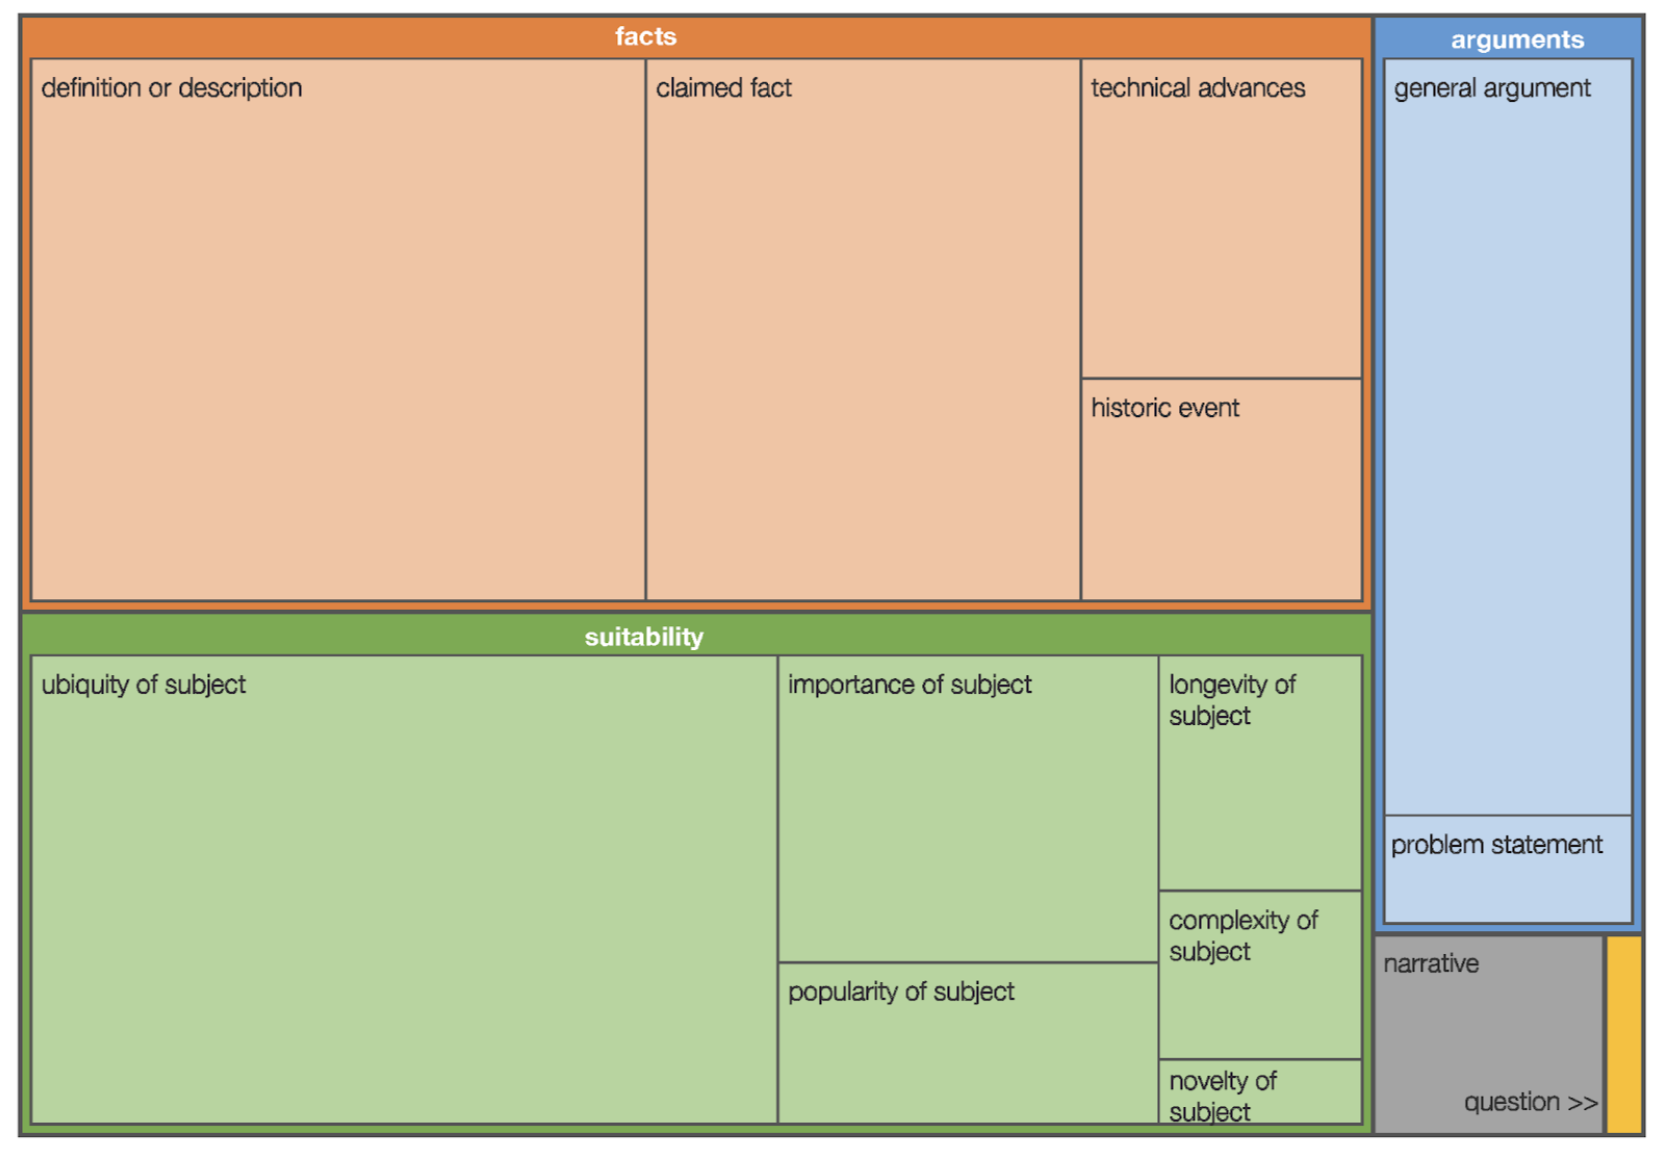
\includegraphics[width=0.8\textwidth]{image.png}
	\caption{A treemap of our codes for the opening sentences of 379 research papers. The size (in area) of each visualized code is proportional to the number of sentences with that code.}
	\label{fig:treemap}
\end{figure*}
	
	
	
	Figure~\ref{fig:treemap} shows the taxonomy of our codes where the area of the box is proportional to how many times they were used. We provide a description of each category, as well as several examples, later in this section.
	
	To arrive at this figure, we followed the coding techniques of grounded theory assisted by the qualitative analysis software tool NVIVO. The process consisted of first partitioning out the opening sentence of each paper. We read many sentences without coding them to have an initial sense of the variety of sentences. We then started `open coding' by creating codes that were as general as possible. Roughly every 50 papers, we would review only the papers with a specific code and try to sub-categorize them (`code upon'), while also vetting the codes and moving papers to other codes as needed. We also re-categorized the codes many times (`axial coding'), eventually arriving at Figure~\ref{fig:treemap}. We did a final code-by-code pass to ensure all the sentences matched the code description and were coherent with each other. 
	
	Grounded theory has a natural halting condition when no new codes are observed, and we halted after three years of proceedings. That is not to say that our categorization does not miss other kinds of sentences, only that new kinds should be rare if the dataset is representative. The final step of grounded theory is to pull general theories out of the codes and their categorization, which we do not pursue since our end goal was classification. We also were not coding the \textit{content} of the sentences, only the kind of writing they exhibit. For these reasons, we emphasize that we used the coding techniques of grounded theory rather than exactly grounded theory itself. 
		
	One further note about citations: we do not include individual citations to the paper that each sentence is extracted from, as the bibliography for this paper would exceed the page limit. The sentences are from the following three proceedings: \textblue{cite the USENIX proceedings as a whole}. A full length version of this paper is available with individual citations (linked remove for anonymity). Finally, several quoted sentences have citations embedded within them. We leave these quoted verbatium, noting that the citation numbers within the quoted sentences are relevant to the context of the quoted paper and make no reference to the bibliography of this paper. 
	
	
	\subsection{Facts}
	\subsubsection{Facts: Definition or Description}
	
	Many papers start with a straightforward definition of the subject of the paper. These tend to be neutral and like something you would read in a glossary.
	
	\begin{itemize}
		
		\item	``Malware sandboxes are automated dynamic analysis tools that execute samples in an isolated and instrumented environment.''
		
		\item	``Secure two-party computation allows two parties to process their sensitive data in such a way that its privacy is protected.''
		
		\item	``HMAC is a cryptographic authentication algorithm, the ‘Keyed-Hash Message Authentication Code,’ widely used in conjunction with the SHA-256 cryptographic hashing primitive.''
		
	\end{itemize} 
	
	Similarly, papers might provide a description of what the subject of a sentence does or how it works. These are also neutral statements and like something you’d read in a textbook. 
	
	\begin{itemize}
		
		\item	``Traditionally, digital investigations have aimed to recover evidence of a cyber-crime or perform incident response via analysis of non-volatile storage.''
		
		\item	``Mobile social applications discover nearby users and provide services based on user activity (what the user is doing) and context (who and what is nearby).''
		
		\item	``To reduce the memory footprint of a system, the system software shares identical memory pages between processes running on the system.''
	\end{itemize} 	
	\subsubsection{Facts: Claimed Fact}
	
	Another neutral approach to an opening sentence is to provide a fact that is relevant to the subject of the paper. Later we will discuss arguments which are often expressed as if they are facts but are only debatably true. A claimed fact’s correctness should either be apparent or at least provable (i.e., falsifiable). 
	\begin{itemize}	
		\item	``Users are often advised or required to choose passwords that comply with certain policies.''
		
		\item	``Mobile apps frequently demand access to private information.''
		
		\item	``For several decades, car keys have been used to physically secure vehicles.''
		
		\item	``Some sentences use stronger and more vivid language but are still factually based.'' 
		
		\item	``In spite of extensive industrial and academic efforts (e.g., [3, 41, 42]), distributed denial-of-service (DDoS) attacks continue to plague the Internet.''
	\end{itemize} 		
	\subsubsection{Facts: Technical Advances}
	
	Many opening sentences lay out a technical advance in the subject of the sentence. This creates a window of opportunity for the researcher to later identify a novel research problem caused by the changing technology.  It is common to see words like: evolve, become, transition, and improve.
	\begin{itemize}		
		\item	``Recent advances in cloud computing enable customers to outsource their computing tasks to the cloud service providers (CSPs).''
		
		\item	``Browsers have evolved over recent years to mediate a wealth of user interactions with sensitive data.''
		
		\item	``Since its beginning in the early nineties, the Web evolved from a mechanism to publish and link static documents into a sophisticated platform for distributed Web applications.''
	\end{itemize} 		
	\subsubsection{Facts: Historic Events}
	
	A final type of neutral opening sentence will refer to some historic event. 
	\begin{itemize} 		
		\item	``In 1996, Wagner and Schneier performed an analysis of the SSL 3.0 protocol [67].''
		
		\item	``In February 2011, a new Tor hidden service [16], called “Silk Road,” opened its doors.''
		
		\item	``The Network Time Protocol (NTP) is one of the Internet’s oldest protocols, dating back to RFC 958 [15] published in 1985.''
	\end{itemize} 		
	In some cases, a paper opens with a “compound” sentence that makes reference to a historic event in one clause of the sentence, while having additional clauses of a different category. For example, the following sentence refers to a historic event as well as a technical advance.
	
	\begin{itemize}
		\item 	``Starting from Denning’s seminal work in 1986 [9], intrusion detection has evolved into a number of different approaches.''
	\end{itemize}	
	
	
	\subsection{Arguments}
	\subsubsection{Arguments: General Argument}
	
	Many opening sentences issue a subjective argument that represents the authors’ opinion. Unlike a fact, it isn’t straightforward that the reader will accept it as true. While arguments are less neutral than facts, they can be more interesting and provocative, which can help draw the reader into the paper.
	
	The arguments we categorize under “general arguments” do not fit elsewhere in our categorization system. As we go through more categories, we will see other more specific kinds of arguments. 
	\begin{itemize}
		\item ``It is a truth universally acknowledged, that password-based authentication on the web is insecure.''
		
		\item 	``The dismissal of human memory by the security community reached the point of parody long ago.''
		
		\item ``In recent years, unwanted software has risen to the forefront of threats facing users.''
		
		\item 		``The phenomenal growth of Android devices brings in a vibrant application ecosystem.''
	\end{itemize}
	
	
	\subsubsection{Arguments: Problem Statement }
	
	A special type of argument is a “problem statement” which uses the opening sentence to establish a problem or challenge to be solved. 
	\begin{itemize}
		\item ``A key challenge when running untrusted virtual machines is providing them with efficient and secure I/O.''
		
		\item``Determining the semantic similarity between two pieces of binary code is a central problem in a number of security settings.''
		
		\item``It is difficult to keep secrets during program execution.''
		
		
	\end{itemize}
	
	For some sentences, the problem is not stated explicitly but can be inferred from what is said. For example, the “pressure to respond” in the following sentence implies a problem.
	\begin{itemize}
		\item ``As popular applications rely on personal, privacy-sensitive information about users, factors such as legal regulations, industry self-regulation, and a growing body of privacy-conscious users all pressure developers to respond to demands for privacy.''
	\end{itemize}
	
	
	\subsection{Suitability}
	\subsubsection{Suitability: Importance of subject}
	
	A large set of sentences make a special kind of argument: that the subject of the opening sentence is suitable or worthy of research. The exact reasons they are suitable fall into a few sub-categories: the subject is important, ubiquitous, complex, novel, popular with other researchers, or has been around a long time. 
	
	Many opening sentences state that their subject is important, with the implication that it is thus suitable for research.
	\begin{itemize}
		\item 	``Security has now become an important and real concern to connected and/or automated vehicles.''
		
		\item 	``Error handling is an important aspect of software development.''
		
		\item 	``SSL/TLS is, due to its enormous importance, a major target for attacks.''
	\end{itemize}
	
	
	Some sentences do not explicitly use the word “important” but find other ways to convey the same notion. For example, a concern or component might be described as essential or crucial or serious.
	\begin{itemize}
		\item 	``The threat of data theft in public and private clouds from insiders (e.g. curious administrators) is a serious concern.''
		
		\item 	``The same-origin policy (SOP) is a cornerstone of web security, guarding the web content of one domain from the access from another domain."
	\end{itemize}
	
	
	\subsubsection{Suitability: Ubiquity of subject}
	
	The most popular kind of opening sentence argues that a subject is suitable for research because it is ubiquitous and widely used.
	\begin{itemize}
		\item ``Billions of users now depend on online services for sensitive communication.''
		
		\item	``Embedded systems are omnipresent in our everyday life.''
		
		\item	``Android is the major platform for mobile users and mobile app developers.''
	\end{itemize}
	
	
	\subsubsection{Suitability: Popularity of subject}
	
	While the ubiquity of a subject corresponds to how widely it is used, a closely related variant points out that the subject has received a lot of attention. Often, this means attention from other researchers which lends credibility to the subject for further research.
	\begin{itemize}
		\item	``Protecting the privacy of user data within mobile applications (apps for short) has always been at the spotlight of mobile security research.''
		
		\item	``The black-market economy for purchasing Facebook likes, Twitter followers, and Yelp and Amazon reviews has been widely acknowledged in both industry and academia [6, 27, 37, 58, 59].''
		
		\item	``Since the first widely-exploited buffer overflow used by the 1998 Morris worm [27], the prevention, exploitation, and mitigation of memory corruption vulnerabilities have occupied the time of security researchers and cybercriminals alike.''
	\end{itemize}
	\subsubsection{Suitability: Longevity of subject }
	
	In this category, how long a subject has been around is the key component to why it is a suitable subject for study. In some cases, a specific duration is provided and in others, it is implied that the amount of time is significant.
	\begin{itemize}
		\item ``Redaction of sensitive information from documents has been used since ancient times as a means of concealing and removing secrets from texts intended for public release.''
		
		\item	``Since its beginning in the early nineties, the Web evolved from a mechanism to publish and link static documents into a sophisticated platform for distributed Web applications.''
	\end{itemize}
	
	
	\subsubsection{Suitability: Complexity of subject}
	
	In this category, the complexity of the subject is highlighted, implying that the complexity creates new issues or requires further research. The complexity might be inherent to the subject itself. Or there might be a complex set of external factors to consider.
	\begin{itemize}
		\item 	``Today, large and complex software is built with many components integrated using APIs.''
		
		\item ``The capabilities and limitations of disassembly are not always clearly defined or understood, making it difficult for researchers and reviewers to judge the practical feasibility of techniques based on it.''
		
		\item 	``As popular applications rely on personal, privacy-sensitive information about users, factors such as legal regulations, industry self-regulation, and a growing body of privacy-conscious users all pressure developers to respond to demands for privacy.''
	\end{itemize}
	
	
	\subsubsection{Suitability: Novelty of subject}
	
	Finally, a degree of novelty is an important component in any research question so it is unsurprising that papers begin arguing novelty from their opening sentence. In this category, sentences focus on something that is new or emerging. 
	\begin{itemize}
		\item 	``In the last few years, a new class of cyber attacks has emerged that is more targeted at individuals and organizations.''
		
		\item  ``Although the operating system (OS) kernel has always been an appealing target, until recently attackers focused mostly on the exploitation of vulnerabilities in server and client applications— which often run with administrative privileges—as they are (for the most part) less complex to analyze and easier to compromise.''
		
		\item 	``This sentence manages to appeal to both longevity and novelty by relating two subjects.''
		
		\item  ``While cryptocurrency has been studied since the 1980s [22, 25, 28], bitcoin is the first to see widespread adoption.''
		
	\end{itemize}
	
	\subsection{Narrative}
	
	A potentially interesting way to draw a reader into a paper is by establishing a narrative: a scenario that gets the reader thinking about themselves or other people and what they might do.  
	\begin{itemize}
		\item 	``Consider that you are a domain owner, holding a few domain names that you do not have a better use of.''
		
		\item 	``Consider the setting where a client owns a public input x, a server owns a private input w, and the client wishes to learn z := F(x,w) for a program F known to both parties.''
		
		\item 	``Narratives might also set a scene, like the academic version of an “establishing shot” from films and TV. ''
		
		\item 	``Our phones are always within reach and their location is mostly the same as our location.''
		
		\item 	``We live in a “big data” world.''
		
		\item 	``The battle for the living room is in full swing.''
	\end{itemize}
	
	
	\subsection{Question} 
	
	Making the reader curious is another good way to begin a paper, and this can be accomplished using a question. In our sample, this was underused with only one example.
	\begin{itemize}
		\item ``Do programmers leave fingerprints in their source code?''
	\end{itemize}
	
	\section{Discussion}
One of the questions we asked was ``Do you have to be an expert in security\&privacy to understand these opening sentences? ''. The way the opening sentence is constructed changes the audience that it targets. Let's consider this opening sentence: ``The widespread adoption of DEP, which ensures that all writable pages in memory are nonexecutable, has largely killed classic code injection attacks.'' When one looks at this example, even though they are not an expert (and they don't know what DEP or code injection attack is), they can still understand the gist of it. One would associate the word attack with negative outcomes and would decide that the fact``DEP has killed classic code injection attacks'' is something good and preferred. But what if the sentence was like this: ``The widespread adoption of DEP, which ensures that all writable pages in memory are nonexecutable, has largely killed classic code injection.'' Then, here we need the expertise. The reader has to know that code injection is a type of attack, so the message is correctly conveyed to the reader. For a person who is not an expert in the area it is not cleat whether classic code injection being killed is a desirable property or not.


\textblue{Mention the following are secondary codes?}

We also analyzed to what extend the authors add ``colour commentary'' in the opening sentence. The decision to use this type of commentary is related to how researchers perceive and define the `seriousness' of the topic: Is avoiding some colour in the text a way to prove that the problem they are working on is significant and should be taken seriously? To add some colour, some papers use rhetoric to make a point. What makes these sentences more vivid is the rich choice of words (``The defacement and vandalism of websites is an attack that disrupts the operation of companies and organizations, tarnishes their brand, and plagues websites of all sizes, from those of large corporations to the websites of single individuals;'' ``The dismissal of human memory by the security community reached the point of parody long ago;'' ``Video is ineffably compelling''). We also not that the colour commentary in these sentences cannot be characterized as``purple prose'', which defines an ornate and elaborate writing. 

As for the length of the opening sentence, we compered the shortest and longest ones to discuss their properties. Short sentences are striking and easy to remember. The shortest ones from our data set were four words long: ``Video is ineffably compelling'' and ``Software bugs are expensive.'' Long sentences can obviously convey more information or make a complex argument, but they might have to be read a few times to fully parse what they are saying. King has a similar argument in~\cite{king1967opening}, where he gives an example of a long opening sentence in medical writing and he simplifies the sentence by shortening it and as a result making it more concise and easier to parse.

Appealing to the notion that a domain is important because of its longevity is also a common way to start a paper in our data set. The idea of appealing to years or decades of work is extremely common (``Over the last few years there have been numerous reports…'' ``The last decade in cryptography…'' ``Over the past few years, face authentication systems…'' ``For several decades, car keys…''). 

There was one category of sentences that is specific to security and privacy. In security, you can imagine that researchers want to tackle the biggest threats. Many use their opening sentence to position themselves as such. While some of them directly state that it is the most prevalent threat (``In recent years, unwanted software has risen to the forefront of threats facing users;'' ``Today, runtime attacks remain one of the most prevalent attack vectors against software programs;'' ``Remote malware downloads currently represent the most common infection vector.''), others prefer to make their point in a stronger way with their choice of words (``In spite of extensive industrial and academic efforts (e.g., [3, 41, 42]), distributed denial-of-service (DDoS) attacks continue to plague the Internet'').

	
	\section{Conclusion and Future Work}
	
	As researchers, we often find ourselves staring at the blinking cursor, trying to come up with a witty and neat way to start our paper to engage the audience. The opening sentence has a responsibility because it is a way to be remembered, just like in the novels. Chances are high that you recognize many opening sentences of famous literary works even if you haven’t read them. Knowing how many times we have struggled with an opening sentence, we were curious how other researchers begin their papers. We know every researcher has their own style of telling the story of their research process. 
	
	We also discuss whether a similar classification can be used in other domains or the categories that we present in this paper are domain-specific. And if we can use the same categories, how the weights of these categories differ in other areas.
	
	Future work maybe:
	
	In other domains: categories can completely change or same categories can be used but their weights change.
	
	Maybe in history, political science or economics a similar classification can be used?
	
	But we think that we may need different categories if we do the same study in literature. 
	
	
	We also observe that the opening sentences that we coded are not too elaborate or ornate (this type of writing is defined as `purple prose').
	
	
	
	\bibliographystyle{ACM-Reference-Format}
	\bibliography{acmart}
\end{document}
\endinput
%%
%% End of file `sample-sigconf.tex'.
